%!TEX root = Constructive Alignment for Introductory Programming.tex

\chapter{Introduction} % (fold)
\label{cha:introduction}

% Context, general problem, current solutions, why these solutions are still lacking, broadly what needs to be solved, my focus and research goal (something like that)

Programming is a critical skill in Computer Science and Software Engineering, as a consequence students in these fields are taught programming from the start of their degree programmes at many Universities. Although we have been teaching programming for a number of decades, learning programming remains challenging \cite{Jenkins:2002,Lahtinen:2005,Lister:2004,McCracken:2001,Ragonis:2007,Robins:2003,Rountree:2002,Renumol:2010,Wiedenbeck:2005}, with a general consensus that many students find programming hard. These challenges, along with the current lack of success in this critical area, have been recognied by \citet{McGettrick:2005} as one of their seven grand challenges in computing education. Despite persistent efforts over many years, we are still a long way from having specific guidance on how best to approach teaching introductory programming. 

Research into teaching introductory programming is an active part of the computing education research field. In their survey of literature on introductory programming \citet{Pears:2007} identified four main categories: curricula, pedagogy, language choice, and tool support. Work on curricula has examined how introductory programming fits into the wider university computing curricula, including recommendations for computing curricula by major professional computing societies \cite{CC2001,CC2008}. Computing education research on pedagogy examines the teaching and learning of introductory programming and include work such as approaches to adapt learning theory for computer science \cite{BenAri:2001}, various views of programming as mathematical \cite{Denning:1989,Dijkstra:1989,Hoare:1969}, problem solving \cite{Palumbo:1990}, or from language syntax and features \cite{Robins:2003}, to work on appropriate cognitive structures \cite{Eckerdal:2005,Green:1996,Green:2000,Soloway:1986}. Language and, by association, paradigm choice is also widely studied, with various papers on the programming language to use in teaching introductory programming \cite{Anik:2011,Boszormenyi:1998,Bishop:2006,Brilliant:1996,Howell:2003,Kelleher:2005,Koffman:1988,Maloney:2010,Mannila:2006,Mannila:2006a,Mody:1991,Pendergast:2006,Roberts:1993} to debates on which programming paradigm should be used early in the curricula \cite{Astrachan:2005,Bennedsen:2004,Cooper:2003,Ehlert:2009,Howe:2004,Lister:2006a,Pattis:1993,Reges:2006}. While research on tool support examines the use of software tools specifically designed to support the needs of novice programmers, including work on automated assessment \cite{AlaMutk:2007,Douce:2005}, visualisation \cite{Naps:2002}, programming environments \cite{Gross:2005,Kelleher:2005,Kolling:2003}.

Advancements from general education literature also provide additional advice on underlying theories and practices. This includes works on the scholarship of teaching and learning \cite{Boyer:1990}, approaches to teaching \cite{Martin:2000}, approaches to learning \cite{Marton:1976a,Marton:1984,Entwistle:1991,Trigwell:1991,Trigwell:1999}, and analysis of the learner's experience \cite{Marton:1997}. While seen as beneficial, many of these general education theories need further research, and a greater inclusion in the computing education research discourse in order to determine their effectiveness in relation to teaching introductory programming.

\rv{Approach towards teaching IP are diverse (TODO: provide some examples and cite). However, when considered in terms of students experience of learning to program\ldots} In their study of students' experiences learning to program, \citet{Bruce:2003} categorised the way students engage with learning to program into five categories range from approaches focusing on ``\emph{getting through the unit}'', to approaches aimed at discovering what it means to be a programmer. Each of these categories can be broadly classified as either a surface or deep approach to learning \cite{Marton:1976a,Ramsden:1992} to program. When engaging surface approaches, students attempt to address the outcomes with as little effort as possible. This leads to situations in which students are primarily motivated by fear of failing, and experience the learning as a struggle, with the topic appearing tedious, hard and boring, adjectives that are too often associated with learning to program \cite{McGettrick:2005}. On the other hand, when engaging deep approaches to learning students seek meaning in what they do, and relate their learning to the bigger picture. To succeed at learning to program, students need to engage deep approaches to learning, as surface approaches alone are unlikely to be sufficient \cite{Bruce:2003}. Pedagogy that encourage students to adopt deep approaches to learning should, therefore, help address some of the issues related to this challenging topic.

Biggs' model of \CA \cite{Biggs:1996c,Biggs:2007}, based upon constructive learning theory (constructivism) and aligned curriculum, aims to enhance student learning outcomes by focusing on \emph{what the student does}. \CA aims to encourage students to use \emph{deep}, rather than \emph{surface}, approaches to learning. The focus on the central role of the learner in building meaning is derived from constructivist learning theories \todo{cite}, whilst the alignment of assessment, teaching, and learning activities, has its foundation in instructional design literature \cite{Cohen:1987} \todo{cite more}. Biggs' model is student focused, with clear and intentional alignment of assessment, teaching and learning activities, and unit objectives. While there is extensive literature on \CA in the general education literature, it has received little attention in computing eduction research related to teaching introductory programming. 

As a form of outcomes based teaching and learning, \CA involves defining intended learning outcomes using verbs that indicate the required cognitive level students must engage. Assessment of student work is then carried out by evaluating the Structure of the Observed Learning Outcome (SOLO), using the SOLO Taxonomy developed by \citet{Biggs:1982}. \fref{constructive_alignment} illustrates the constructive alignment model presented by~\citet{Houghton:2004}, which consists of the following blocks:

\begin{itemize}
  \item \emph{Intended learning outcomes} clearly define required learning in terms of ``performances of understanding''.
  \item \emph{Performance objectives} emerge from the desired outcomes, and can be ranked to become the assessment criteria.
  \item \emph{Teaching and learning activities} are designed to place students in situations likely to elicit the required learning.
  \item Students provide \emph{evidence of their learning}, that is assessed against the criteria to determine grade outcomes.
\end{itemize}

\begin{figure}[htbp]
  \centering
  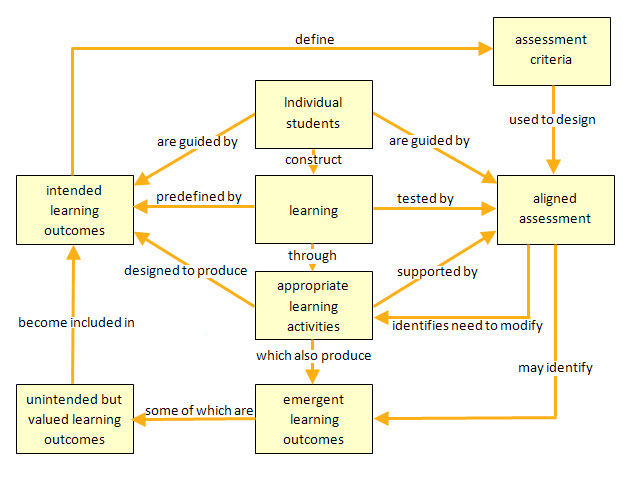
\includegraphics[width=\textwidth]{Houghton_constructive_alignment_1}
  \caption{Constructive alignment model presented by ~\citet{Houghton:2004}}
  \label{fig:constructive_alignment}
\end{figure}

% Teaching environment
Constructive alignment's success relies upon creating an academic environment that fosters deep learning. Interventions that impact on the learning environment, also referred to as teaching or academic environment, have the potential to positively influence student learning outcomes \cite{Trigwell:1991}. Learning environments have been found to influence students' approach to learning \cite{Entwistle:1990,Entwistle:1991,Kember:2007}, and perceptions of teaching environments have been shown to directly, and indirectly, influence learning outcomes \cite{Meyer:1990,Lizzio:2002}.

% Flipped Classroom


% "Meyer and Eley (1999, p. 198) argue that: individual students might well adopt differentiated pattems of learning behaviours that are attributable to the learning contexts shaped by different subjects. That is, perceptions and experiences of learning contexts might be shaped also by the epistemology of a discipline and they might therefore vary considerably from one discipline to another."

Given this context, \todo{describe context}
Research that examines teaching environments is of great importance as it aids to build...


% - image on iterative nature of teaching

\section{Research Goals} % (fold)
\label{sec:research_goals}

This work will look to answer the following question. In what way can \emph{constructive alignment} be applied to the teaching of \emph{introductory programming} to stimulate \emph{deep approaches to learning}?

% To answer this question it is necessary to design and implement an introductory programming subject using the principles of constructive alignment. Designing such a subject requires the definition of intended learning outcomes, a statement of the assessment criteria, aligned teaching and learning activities, and a specific assessment approach. These activities require the following questions to be asked.

% \begin{enumerate}
%   \item What are appropriate intended learning outcomes?
%   \item Given the stated learning objectives, how can assessment criteria be structured to encourage students to use progressively deeper cognitive levels of activity in order to achieve higher grades? (memorise to reflect)
%   \item What teaching and learning activities help create an effective learning environment that encourages deep approaches to learning and a meaningful student experience?
%   \item How can criterion referenced assessment and holistic grading be used to assess student outcomes?
% \end{enumerate}

% To assess the effectiveness of the proposed teaching method the following questions will be addressed.

% \begin{enumerate}
%   \item Does this teaching method change the way students approach learning and/or their work in general?
%   \item What affect does this teaching method have on student engagement?
%   \item Are students able to effectively select material to demonstrate coverage of the intended learning outcomes?
%   \item To what depth does submitted work demonstrate the intended learning outcomes?
%   \item To what degree are students able to correctly assess their work against the subject's assessment criteria?
%   \item How well do students retain the knowledge and skills they develop in the subject?
% \end{enumerate}

% % Improve depth of learning.
% % 
% % Our method of teaching with constructive alignment: 
% % \begin{itemize}
% %   \item Determine learning objectives
% %   \item Create tiered assessment criterion that provide requirements for differing depths of understanding...
% %   \item Make students responsible for as much of their learning as possible. It is what they do that counts.
% %   \item Teach programming, not the language. Focus lectures on concepts and abstractions, provide just enough syntax to get the students started.
% %   \item Provide resources for students to learn the required syntax to map concepts to code (podcasts, text) to allow them to learn independently.
% %   \item Provide regular formative feedback on assessment work
% %   \item Have students prepare a portfolio of their work that demonstrates how they have addressed the assessment criteria
% % \end{itemize}
% % 
% % \bigskip
% % 
% % Guiding principles:
% % \begin{itemize}
% %   \item Truth. Remain true to the language and how it should be used. Avoid half truths as much as possible.
% %   \item Trust. Students are there to learn. They are capable and just need direction, encouragement, and feedback. Theory Y.
% %   \item Construct knowledge. Introduce the concepts needed to fully\footnote{Fully at this level of abstraction.} understand the programs they are writing. Avoid all forms of `magic'.
% %   % \item Students should use deep approaches to learning.
% %   % \item Programs are not sufficient to assess the depth of a students understanding.
% %   \item Maintain a good signal to noise ratio. Provide the essential material and have students explore the details themselves.
% %   \item Encourage deep exploration once concepts are grasped. For example, encourage students to look at how programming mechanisms work like how parameter passing works, how the stack grows, how a program's memory is organised.
% %   \item Flexible delivery with clear learning outcomes that allow students to customise the learning experience to their own needs and interests.
% %   \item Self efficacy allowing students to work toward a grade.
% % \end{itemize}
% % 
% % \clearpage

% % In what way can \emph{constructive alignment} be applied to the teaching of \emph{introductory programming} to stimulate \emph{deep learning}?

% % (Breadth vs depth)
% % 
% % What are the benefits of \emph{constructive alignment} for the teaching of \emph{introductory programming}?
% % 
% % What is the impact of \emph{constructive alignment} on overall computer science curriculum?
% % 
% % Does \emph{constructive alignment} encourage \emph{deep approaches to learning} in introductory programming subjects?




% % \begin{enumerate}
% %   \item How have other educational areas implemented constructive alignment?
% %   
% %   \item What are appropriate learning objectives for an introductory programming subject?
% %   \begin{itemize}
% %     \item What are the related programming concepts and abstractions?
% %     \item Are there established models of these concepts and abstractions?
% %     \item How do the concepts and abstractions map to different programming paradigms and languages?
% %     \item Which of these concepts and abstractions are appropriate for introductory programming subjects? What are the differences for subjects that use an `Objects First' approach versus an `Objects Later' approach? How do the two approaches compare on concept and abstraction coverage?
% %   \end{itemize}
% %   
% %   \item Given the selected learning objectives, how can assessment criteria be structured to encourage students to demonstrate use of progressively deeper cognitive levels in order to achieve higher grades? (memorise to reflect)
% %   \begin{itemize}
% %       \item What are the different cognitive levels of activities related to programming? (Is programming really `application' or just `expression'? e.g. getting it to work does even mean the student can explain why/how it works.) How do these relate to deep and surface approaches? How does this map to the SOLO taxonomy. (Is there work related to this?)
% %     % \item Can tiered assessment criteria be developed to map student outcomes to grade categories for use in criterion referenced assessment? How can these be formulated to encourage students to engage deeper learning approaches for higher grades?
% %     \item Are students aware of what is required to achieve different grades, and how does this change during the semester?
% %     \item What affect does the tiered assessment criteria and criterion referenced assessment have on student approaches to learning?
% %     \item Do students use criterion referenced assessment to customise the learning experience to their own requirements,  interests, and aspirations?
% %     \item Does this self directed learning and self efficacy help motivate students? Does this in turn lead to deeper approaches to learning and deeper learning outcomes?
% %     \item How do student aspirations change as the semester progresses? 
% %   \end{itemize}
% %   
% %   % \item What teaching and learning activities can help support the students to studying sound combination of theory and practice.
% %   % \item What benefits are there from providing flexible teaching and learning activities that align with the selected learning outcomes?
% %   % \item Given the selected learning outcomes, what are the benefits of providing flexible teaching and learning activities?
% %   % \item What teaching and learning activities that support and motivate
% %   % 
% %   % \item What teaching and learning activities help support student self-directed leaning of the conten
% %   % 
% %   % \item Can innovative teaching and learning activities encourage students to use deep approaches to learning?
% %   % 
% %   % \item Given the learning objective and assessment criteria, what teaching and learning activities are effective/ineffective?
% %   % 
% %   % \item What do students find useful about the teaching and learning activities used?
% %   
% %   % \item What teaching and learning activities can create an effective learning environment and a meaningful student experience?
% %   
% %   \item What teaching and learning activities help create an effective learning environment and meaningful student experience?
% %   \begin{enumerate}
% %     \item How can we make more effective use of lecture time? 
% %     \item Can we focus on programming concepts and abstractions at a higher level and use other means to cover details of language syntax?
% %     \item Can language syntax be covered sufficiently if the lecture focus shifts toward concepts?
% %     \item What effect does this have on student learning outcomes, sense of achievement, and learning approach?
% %     \item Are video podcasts an effective means of demonstrating programming abstractions and syntax?
% %     \item Does the focus on concepts help students learn a second programming language? How?
% %     \item How much overhead is there in switching between languages?
% %     \item Can you effectively teach programming using multiple languages in the one subject? What are the advantages and disadvantages of this?
% %     \item How does covering multiple languages impact on the student's learning experience?
% %     
% %     \item Will students use a focused episodic text? (??)
% %     % \item Motivation (Dan Pink, Motivation)
% %     \item Self determination (efficacy)
% %   \end{enumerate}
% %   
% %   % Holistic, 
% %   % Formative assessment during the semester
% %   
% %   \item How can criterion referenced assessment and holistic grading be used as assess student outcomes in introductory programming subjects?
% %   % \item Can portfolio assessment be used effectively for assessing student outcomes in introductory programming subjects?
% %   \begin{enumerate}
% %     \item What benefits are there from this approach to assessment and grading?
% %     \begin{itemize}
% %       \item Self efficacy?
% %       \item Deep learning outcomes?
% %     \end{itemize}
% %     \item What mechanisms can be introduced to limit plagiarism?
% %     \item Does the use of ungraded formative assessment during semester reduce plagiarism?
% %     \item Are students able to grasp the 
% %     \item What strategies work effectively for providing frequent formative feedback for large classes?
% %     \item What about the portfolio assessment approach encourages or discourages plagiarism? What mechanisms can be put in place to further discourage plagiarism?
% %     
% %     \item How are student portfolios affected by the statement of the assessment criteria?
% %     \item Does criterion referenced assessment alter the way students approach study in the subject?
% %     \item Does criterion referenced assessment alter the way students approach study in other subjects?
% %     \item Does their approach to portfolio assessment change in subsequent subjects that use the same approach? How? How do these changes (if there are any) relate to deep approaches to learning?
% %     \item Can portfolio assessment be scaled to larger class sizes?
% %   \end{enumerate}
% %   
% %   \item How do student approaches to learning change over time?
% %   \begin{enumerate}
% %     \item During the semester
% %     \item Over the year
% %     \item Across the course
% %     \item After uni
% %   \end{enumerate}
% %   
% %   \item What makes this an effective or ineffective method of teaching introductory programming?
% %   \item What effect does this teaching method have on student graduate attributes? (communication, problem solving, etc.)
% %   
% % \end{enumerate}
% % 
% % Objective:
% % \begin{enumerate}
% %   \item Model of programming concepts and abstractions, with multiple views for different language and paradigms.
% %   \item Guidelines on programming concepts applicable for introductory programming.
% %   \item Guidelines for building tiered assessment criteria.
% %   \item Guidelines, support for, benefits of constructive alignments etc.
% %   \item Behaviour tree for diagnostic view when students incorrectly self assess their grade - what was the cause. Student incorrectly self assessed -> over/under -> etc. Vs our expectations vs assessment criteria (grade)
% % \end{enumerate}

% section research_goals (end)


\section{Research Approach} % (fold)
\label{sec:research_approach}

% Research Questions and Method

% section research_approach (end)

\clearpage
\section{Key Contributions} % (fold)
\label{sec:key_contributions}


% In relation to education, this work provides contributions on the application of constructive alignment for teaching and learning. In relation to computer science and software engineering, the contributions include a curriculum based in constructive alignment and supporting tools to enable its implementation and delivery. Together these contributions relate to a teaching and learning context, and therefore the evaluation of this context provides contributions to both fields. 

The contributions of this thesis relate to the dual fields in computing education research: education, and computer science and software engineering (CSSE). This thesis makes the following contributions to the field of education:
\begin{itemize}
	\item An extensive literature review of applications of constructive alignment.
	\item An approach to constructive alignment with strong links to constructivism in both teaching and learning activities, and assessment.
	\item Evaluation of the resulting teaching and learning context from an educational perspective. 
\end{itemize}

% Additionally, this thesis makes a number of contributions to the body of knowledge related to software engineering and computer science:
This thesis makes the following contributions to CSSE:
\begin{itemize}
	\item An introductory programming curriculum designed using the principles of constructive alignment.
	\item A simplified taxonomy of programming concepts, and their use in framing the curriculum.
	\item The structure and implementation of a game development framework designed primarily for teaching introductory programming using the proposed curriculum.
	\item Evaluation of the student learning outcomes in terms of their technical capability and ability to met the intended learning outcomes.
\end{itemize}

As a whole, these contributions support \citet{Biggs:1996c} model of constructive alignment, and demonstrate a learning context that is aptly captured in the following quote \citep{Biggs:2007} (p54):

\begin{quote}
	All components in the system address the same agenda and support each other. The students are `entrapped' in this web of consistency, optimizing the likelihood that they will engage the appropriate learning activities \ldots but leaving them free to construct their knowledge their way.
\end{quote}

% section key_findings (end)


\section{Thesis Structure} % (fold)
\label{sec:thesis_structure}

This thesis first considers the existing applications of constructive alignment, and then goes on to develop a model of constructive alignment using portfolio assessment. Following this a curriculum for introductory programming is proposed, evaluated, and discussed in detail. The remainder of this section describes each of these areas in more detail. 

\textbf{\cref{background} - \cnref{background}} provides an extensive literature review of applications of constructive alignment. The main finding of this work indicates that applications of constructive alignment reported in the research literature tend to focus on aligned curriculum, with constructivism being weakly applied, if at all. Staff aligned teaching and learning activities to intended learning outcomes and assessment. Constructive learning theories, when addressed, related to the design of teaching and learning activities, but not to assessment approach.

\textbf{\cref{approaching_constructive_alignment_with_portfolio_assessment} - \cnref{approaching_constructive_alignment_with_portfolio_assessment}} presents an approach to constructive alignment with strong links to constructivism in both teaching and learning activities, and assessment. While the approach presented was developed for the teaching of introductory programming, general methods for its adoption are presented. This work helps address the gap identified in the literature review.

\textbf{\cref{constructively_aligned_introductory_programming_curriculum} - \cnref{constructively_aligned_introductory_programming_curriculum}} proposes an introductory programming curriculum designed using the principles of constructive alignment, with strong emphasis on both constructivism and aligned curriculum. This curriculum revives the procedures first approach to introductory programming, and moves the focus from syntax to underlying concepts and abstractions. Through the use of graphical programming grammars, the curriculum incrementally introduces students to programming concepts and then associated syntax. This approach is based on constructive learning theories and aims to help students build viable models of the underlying machine and programming abstractions. 
 
\cref{constructively_aligned_introductory_programming_curriculum} also describes a simplified taxonomy of programming concepts. The aim of this taxonomy is to help frame the curriculum and to provide students with a context from which to approach their studies, and provide staff with a framework through which to communicate the programming concepts. An explanation of the taxonomy, and how it relates to introductory programming concepts is presented.

\textbf{\cref{supporting_the_curriculum} - \cnref{supporting_the_curriculum}} describes a game development framework that provides support for the proposed curriculum. This framework was designed primarily as a teaching tool, and secondly for the development of 2D arcade style games. The relationship between the framework, curriculum, and programming concepts is described along with an evaluation of how students make use of these in their assessed work.

\textbf{\cref{evaluation} - \cnref{evaluation}} provides an evaluation of the teaching and learning context created through the implementation of the approach presented. This work examines the resulting learning environment from an education and CSSE perspective. The learning environment was rated highly by students, and there was evidence that most students had engaged deeply with the teaching and learning activities. The context was able to scalable to hundreds of students, with academics needing to spend little time on administration and summative assessment, once the system had been put in place. In terms of student outcomes, grades were at least as good as previous approaches but with the advantage that these results are more clearly aligned to the intended learning outcomes. The importance of this alignment, in addition to its educational benefits, is now paramount, as accreditation bodies look to verify that students have met the stated unit and course learning outcomes. 

% Examination of student work showed that students were able to implement supplied designs, with higher grades indicating the ability to design and implement programs. The focus of the curriculum on concepts over syntax is highlighted in the issues raised in student reflections. The issues from these reflections related primarily to learning in general, with fewer issues on programming topics. When students did comment on issues related to programming they the majority were related to understanding concepts, with few students raising issues directly related to syntax in their reflections. Overall, students were able to demonstrate the intended learning outcomes including explaining programming concepts, using programming grammars to learn languages, and the use of these languages to develop programs.

% An analysis of staff time spent on summative and formative assessment indicated that, with this approach, the majority of assessment time is spent on formative tasks that directly support student learning. At the same time, the summative assessment is able to be carried out quickly and efficiently using feedback generated from the frequent formative feedback. This results in staff being able to focus on helping students develop the intended learning outcomes.

\textbf{\cref{discussion} - \cnref{discussion}} elaborates on the implications of the earlier findings, and how these can apply to wider contexts. This discusses the value of formative assessment and learning through mistakes, various student persona identified through rigorous application of constructive alignment, and challenges facing more wide spread adoption of this approach. This chapter concludes with a discussion of future work aimed at extending the approach and curriculum presented.

\textbf{\cref{conclusion} - \cnref{conclusion}} provides a summary of the thesis, and argues that the findings presented can aid in the design and delivery of teaching and learning in higher education. 

\textbf{The Appendix} contains published versions of this work already published including:
\begin{itemize}
	\item TALE
	\item ACE
	\item ...
\end{itemize}

% section thesis_structure (end)


% chapter introduction (end)

